% Created by tikzDevice version 0.12.3.1 on 2022-03-23 09:57:04
% !TEX encoding = UTF-8 Unicode
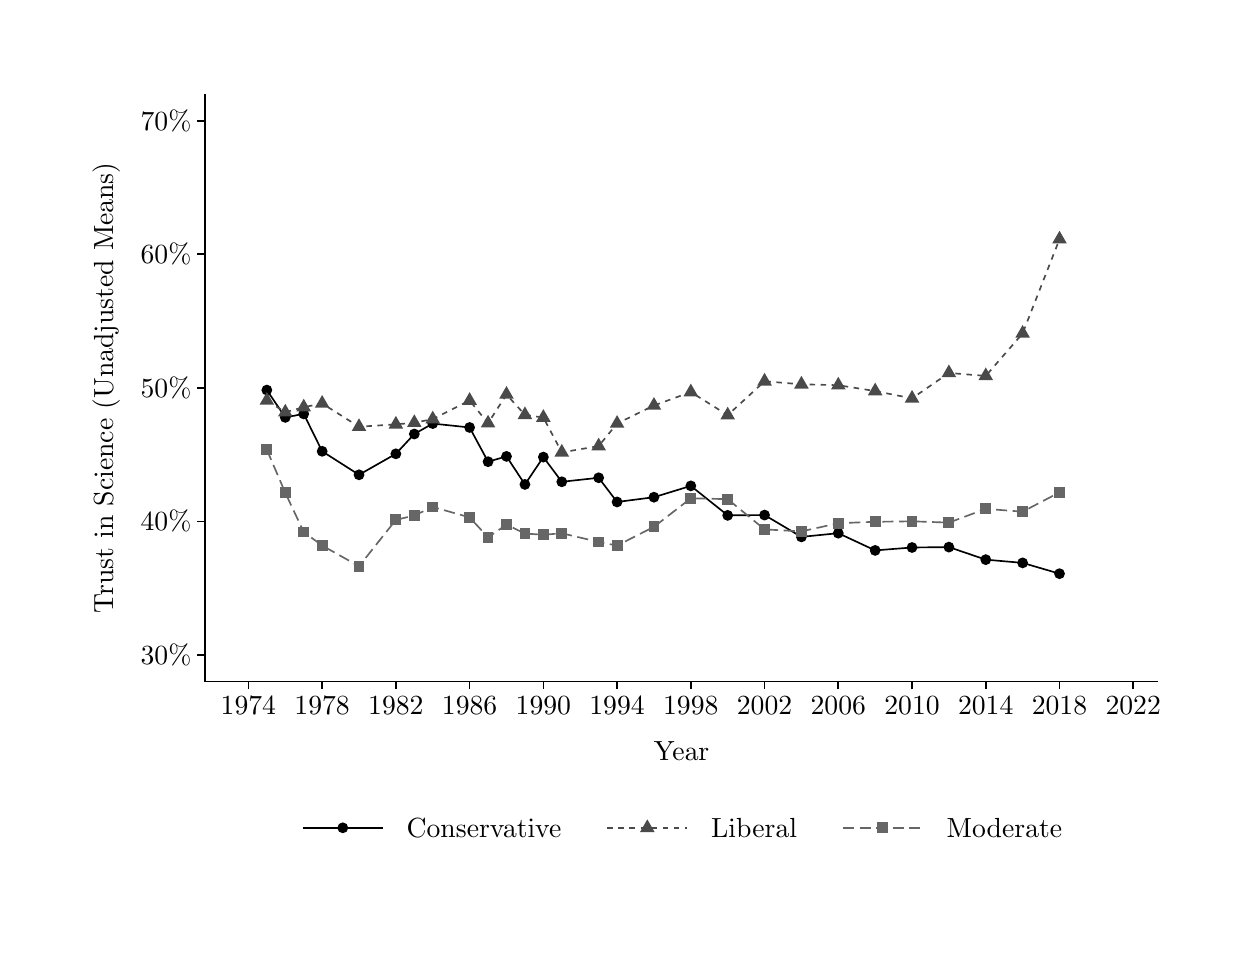
\begin{tikzpicture}[x=1pt,y=1pt]
\definecolor{fillColor}{RGB}{255,255,255}
\path[use as bounding box,fill=fillColor,fill opacity=0.00] (0,0) rectangle (432.48,324.36);
\begin{scope}
\path[clip] (  0.00,  0.00) rectangle (432.48,324.36);
\definecolor{fillColor}{RGB}{255,255,255}

\path[fill=fillColor] ( -0.00,  0.00) rectangle (432.48,324.36);
\end{scope}
\begin{scope}
\path[clip] ( 64.11, 88.07) rectangle (408.48,300.36);
\definecolor{fillColor}{RGB}{255,255,255}

\path[fill=fillColor] ( 64.11, 88.07) rectangle (408.48,300.36);
\definecolor{drawColor}{RGB}{0,0,0}

\path[draw=drawColor,line width= 0.6pt,line join=round] ( 86.42,193.40) --
	( 93.09,183.53) --
	( 99.75,184.79) --
	(106.41,171.28) --
	(119.73,162.79) --
	(133.05,170.37) --
	(139.71,177.53) --
	(146.37,181.30) --
	(159.69,179.89) --
	(166.36,167.52) --
	(173.02,169.44) --
	(179.68,159.31) --
	(186.34,169.19) --
	(193.00,160.26) --
	(206.32,161.71) --
	(212.98,152.97) --
	(226.30,154.69) --
	(239.63,158.78) --
	(252.95,148.13) --
	(266.27,148.24) --
	(279.59,140.35) --
	(292.91,141.69) --
	(306.24,135.47) --
	(319.56,136.52) --
	(332.88,136.66) --
	(346.20,132.13) --
	(359.52,130.96) --
	(372.85,127.06);
\definecolor{drawColor}{gray}{0.29}

\path[draw=drawColor,line width= 0.6pt,dash pattern=on 2pt off 2pt ,line join=round] ( 86.42,189.63) --
	( 93.09,185.39) --
	( 99.75,187.23) --
	(106.41,188.56) --
	(119.73,180.16) --
	(133.05,181.02) --
	(139.71,181.59) --
	(146.37,182.92) --
	(159.69,189.61) --
	(166.36,181.42) --
	(173.02,191.80) --
	(179.68,184.47) --
	(186.34,183.48) --
	(193.00,170.90) --
	(206.32,173.16) --
	(212.98,181.31) --
	(226.30,187.83) --
	(239.63,192.68) --
	(252.95,184.34) --
	(266.27,196.58) --
	(279.59,195.49) --
	(292.91,195.16) --
	(306.24,193.05) --
	(319.56,190.40) --
	(332.88,199.59) --
	(346.20,198.52) --
	(359.52,213.87) --
	(372.85,247.92);
\definecolor{drawColor}{gray}{0.40}

\path[draw=drawColor,line width= 0.6pt,dash pattern=on 4pt off 2pt ,line join=round] ( 86.42,171.86) --
	( 93.09,156.28) --
	( 99.75,142.11) --
	(106.41,137.23) --
	(119.73,129.74) --
	(133.05,146.50) --
	(139.71,148.08) --
	(146.37,151.17) --
	(159.69,147.40) --
	(166.36,140.20) --
	(173.02,144.78) --
	(179.68,141.56) --
	(186.34,141.12) --
	(193.00,141.66) --
	(206.32,138.53) --
	(212.98,137.20) --
	(226.30,143.98) --
	(239.63,154.30) --
	(252.95,153.99) --
	(266.27,143.06) --
	(279.59,142.34) --
	(292.91,145.29) --
	(306.24,145.81) --
	(319.56,145.98) --
	(332.88,145.51) --
	(346.20,150.48) --
	(359.52,149.46) --
	(372.85,156.44);
\definecolor{fillColor}{RGB}{0,0,0}

\path[fill=fillColor] ( 86.42,193.40) circle (  1.96);
\definecolor{fillColor}{gray}{0.29}

\path[fill=fillColor] ( 86.42,192.68) --
	( 89.07,188.11) --
	( 83.78,188.11) --
	cycle;
\definecolor{fillColor}{gray}{0.40}

\path[fill=fillColor] ( 84.46,169.89) --
	( 88.39,169.89) --
	( 88.39,173.82) --
	( 84.46,173.82) --
	cycle;
\definecolor{fillColor}{RGB}{0,0,0}

\path[fill=fillColor] ( 93.09,183.53) circle (  1.96);
\definecolor{fillColor}{gray}{0.29}

\path[fill=fillColor] ( 93.09,188.44) --
	( 95.73,183.86) --
	( 90.44,183.86) --
	cycle;
\definecolor{fillColor}{gray}{0.40}

\path[fill=fillColor] ( 91.12,154.32) --
	( 95.05,154.32) --
	( 95.05,158.24) --
	( 91.12,158.24) --
	cycle;
\definecolor{fillColor}{RGB}{0,0,0}

\path[fill=fillColor] ( 99.75,184.79) circle (  1.96);
\definecolor{fillColor}{gray}{0.29}

\path[fill=fillColor] ( 99.75,190.28) --
	(102.39,185.70) --
	( 97.10,185.70) --
	cycle;
\definecolor{fillColor}{gray}{0.40}

\path[fill=fillColor] ( 97.78,140.14) --
	(101.71,140.14) --
	(101.71,144.07) --
	( 97.78,144.07) --
	cycle;
\definecolor{fillColor}{RGB}{0,0,0}

\path[fill=fillColor] (106.41,171.28) circle (  1.96);
\definecolor{fillColor}{gray}{0.29}

\path[fill=fillColor] (106.41,191.62) --
	(109.05,187.04) --
	(103.76,187.04) --
	cycle;
\definecolor{fillColor}{gray}{0.40}

\path[fill=fillColor] (104.45,135.27) --
	(108.37,135.27) --
	(108.37,139.19) --
	(104.45,139.19) --
	cycle;
\definecolor{fillColor}{RGB}{0,0,0}

\path[fill=fillColor] (119.73,162.79) circle (  1.96);
\definecolor{fillColor}{gray}{0.29}

\path[fill=fillColor] (119.73,183.21) --
	(122.37,178.63) --
	(117.09,178.63) --
	cycle;
\definecolor{fillColor}{gray}{0.40}

\path[fill=fillColor] (117.77,127.78) --
	(121.69,127.78) --
	(121.69,131.70) --
	(117.77,131.70) --
	cycle;
\definecolor{fillColor}{RGB}{0,0,0}

\path[fill=fillColor] (133.05,170.37) circle (  1.96);
\definecolor{fillColor}{gray}{0.29}

\path[fill=fillColor] (133.05,184.07) --
	(135.69,179.49) --
	(130.41,179.49) --
	cycle;
\definecolor{fillColor}{gray}{0.40}

\path[fill=fillColor] (131.09,144.54) --
	(135.01,144.54) --
	(135.01,148.46) --
	(131.09,148.46) --
	cycle;
\definecolor{fillColor}{RGB}{0,0,0}

\path[fill=fillColor] (139.71,177.53) circle (  1.96);
\definecolor{fillColor}{gray}{0.29}

\path[fill=fillColor] (139.71,184.65) --
	(142.35,180.07) --
	(137.07,180.07) --
	cycle;
\definecolor{fillColor}{gray}{0.40}

\path[fill=fillColor] (137.75,146.11) --
	(141.67,146.11) --
	(141.67,150.04) --
	(137.75,150.04) --
	cycle;
\definecolor{fillColor}{RGB}{0,0,0}

\path[fill=fillColor] (146.37,181.30) circle (  1.96);
\definecolor{fillColor}{gray}{0.29}

\path[fill=fillColor] (146.37,185.97) --
	(149.02,181.39) --
	(143.73,181.39) --
	cycle;
\definecolor{fillColor}{gray}{0.40}

\path[fill=fillColor] (144.41,149.20) --
	(148.34,149.20) --
	(148.34,153.13) --
	(144.41,153.13) --
	cycle;
\definecolor{fillColor}{RGB}{0,0,0}

\path[fill=fillColor] (159.69,179.89) circle (  1.96);
\definecolor{fillColor}{gray}{0.29}

\path[fill=fillColor] (159.69,192.67) --
	(162.34,188.09) --
	(157.05,188.09) --
	cycle;
\definecolor{fillColor}{gray}{0.40}

\path[fill=fillColor] (157.73,145.44) --
	(161.66,145.44) --
	(161.66,149.36) --
	(157.73,149.36) --
	cycle;
\definecolor{fillColor}{RGB}{0,0,0}

\path[fill=fillColor] (166.36,167.52) circle (  1.96);
\definecolor{fillColor}{gray}{0.29}

\path[fill=fillColor] (166.36,184.47) --
	(169.00,179.89) --
	(163.71,179.89) --
	cycle;
\definecolor{fillColor}{gray}{0.40}

\path[fill=fillColor] (164.39,138.23) --
	(168.32,138.23) --
	(168.32,142.16) --
	(164.39,142.16) --
	cycle;
\definecolor{fillColor}{RGB}{0,0,0}

\path[fill=fillColor] (173.02,169.44) circle (  1.96);
\definecolor{fillColor}{gray}{0.29}

\path[fill=fillColor] (173.02,194.86) --
	(175.66,190.28) --
	(170.37,190.28) --
	cycle;
\definecolor{fillColor}{gray}{0.40}

\path[fill=fillColor] (171.05,142.82) --
	(174.98,142.82) --
	(174.98,146.74) --
	(171.05,146.74) --
	cycle;
\definecolor{fillColor}{RGB}{0,0,0}

\path[fill=fillColor] (179.68,159.31) circle (  1.96);
\definecolor{fillColor}{gray}{0.29}

\path[fill=fillColor] (179.68,187.52) --
	(182.32,182.94) --
	(177.04,182.94) --
	cycle;
\definecolor{fillColor}{gray}{0.40}

\path[fill=fillColor] (177.72,139.59) --
	(181.64,139.59) --
	(181.64,143.52) --
	(177.72,143.52) --
	cycle;
\definecolor{fillColor}{RGB}{0,0,0}

\path[fill=fillColor] (186.34,169.19) circle (  1.96);
\definecolor{fillColor}{gray}{0.29}

\path[fill=fillColor] (186.34,186.53) --
	(188.98,181.95) --
	(183.70,181.95) --
	cycle;
\definecolor{fillColor}{gray}{0.40}

\path[fill=fillColor] (184.38,139.16) --
	(188.30,139.16) --
	(188.30,143.08) --
	(184.38,143.08) --
	cycle;
\definecolor{fillColor}{RGB}{0,0,0}

\path[fill=fillColor] (193.00,160.26) circle (  1.96);
\definecolor{fillColor}{gray}{0.29}

\path[fill=fillColor] (193.00,173.96) --
	(195.64,169.38) --
	(190.36,169.38) --
	cycle;
\definecolor{fillColor}{gray}{0.40}

\path[fill=fillColor] (191.04,139.70) --
	(194.96,139.70) --
	(194.96,143.62) --
	(191.04,143.62) --
	cycle;
\definecolor{fillColor}{RGB}{0,0,0}

\path[fill=fillColor] (206.32,161.71) circle (  1.96);
\definecolor{fillColor}{gray}{0.29}

\path[fill=fillColor] (206.32,176.22) --
	(208.96,171.64) --
	(203.68,171.64) --
	cycle;
\definecolor{fillColor}{gray}{0.40}

\path[fill=fillColor] (204.36,136.56) --
	(208.28,136.56) --
	(208.28,140.49) --
	(204.36,140.49) --
	cycle;
\definecolor{fillColor}{RGB}{0,0,0}

\path[fill=fillColor] (212.98,152.97) circle (  1.96);
\definecolor{fillColor}{gray}{0.29}

\path[fill=fillColor] (212.98,184.37) --
	(215.63,179.79) --
	(210.34,179.79) --
	cycle;
\definecolor{fillColor}{gray}{0.40}

\path[fill=fillColor] (211.02,135.24) --
	(214.94,135.24) --
	(214.94,139.16) --
	(211.02,139.16) --
	cycle;
\definecolor{fillColor}{RGB}{0,0,0}

\path[fill=fillColor] (226.30,154.69) circle (  1.96);
\definecolor{fillColor}{gray}{0.29}

\path[fill=fillColor] (226.30,190.88) --
	(228.95,186.30) --
	(223.66,186.30) --
	cycle;
\definecolor{fillColor}{gray}{0.40}

\path[fill=fillColor] (224.34,142.02) --
	(228.27,142.02) --
	(228.27,145.94) --
	(224.34,145.94) --
	cycle;
\definecolor{fillColor}{RGB}{0,0,0}

\path[fill=fillColor] (239.63,158.78) circle (  1.96);
\definecolor{fillColor}{gray}{0.29}

\path[fill=fillColor] (239.63,195.73) --
	(242.27,191.15) --
	(236.98,191.15) --
	cycle;
\definecolor{fillColor}{gray}{0.40}

\path[fill=fillColor] (237.66,152.33) --
	(241.59,152.33) --
	(241.59,156.26) --
	(237.66,156.26) --
	cycle;
\definecolor{fillColor}{RGB}{0,0,0}

\path[fill=fillColor] (252.95,148.13) circle (  1.96);
\definecolor{fillColor}{gray}{0.29}

\path[fill=fillColor] (252.95,187.39) --
	(255.59,182.81) --
	(250.31,182.81) --
	cycle;
\definecolor{fillColor}{gray}{0.40}

\path[fill=fillColor] (250.99,152.02) --
	(254.91,152.02) --
	(254.91,155.95) --
	(250.99,155.95) --
	cycle;
\definecolor{fillColor}{RGB}{0,0,0}

\path[fill=fillColor] (266.27,148.24) circle (  1.96);
\definecolor{fillColor}{gray}{0.29}

\path[fill=fillColor] (266.27,199.63) --
	(268.91,195.05) --
	(263.63,195.05) --
	cycle;
\definecolor{fillColor}{gray}{0.40}

\path[fill=fillColor] (264.31,141.09) --
	(268.23,141.09) --
	(268.23,145.02) --
	(264.31,145.02) --
	cycle;
\definecolor{fillColor}{RGB}{0,0,0}

\path[fill=fillColor] (279.59,140.35) circle (  1.96);
\definecolor{fillColor}{gray}{0.29}

\path[fill=fillColor] (279.59,198.55) --
	(282.23,193.97) --
	(276.95,193.97) --
	cycle;
\definecolor{fillColor}{gray}{0.40}

\path[fill=fillColor] (277.63,140.38) --
	(281.55,140.38) --
	(281.55,144.31) --
	(277.63,144.31) --
	cycle;
\definecolor{fillColor}{RGB}{0,0,0}

\path[fill=fillColor] (292.91,141.69) circle (  1.96);
\definecolor{fillColor}{gray}{0.29}

\path[fill=fillColor] (292.91,198.21) --
	(295.56,193.64) --
	(290.27,193.64) --
	cycle;
\definecolor{fillColor}{gray}{0.40}

\path[fill=fillColor] (290.95,143.33) --
	(294.88,143.33) --
	(294.88,147.25) --
	(290.95,147.25) --
	cycle;
\definecolor{fillColor}{RGB}{0,0,0}

\path[fill=fillColor] (306.24,135.47) circle (  1.96);
\definecolor{fillColor}{gray}{0.29}

\path[fill=fillColor] (306.24,196.10) --
	(308.88,191.52) --
	(303.59,191.52) --
	cycle;
\definecolor{fillColor}{gray}{0.40}

\path[fill=fillColor] (304.27,143.85) --
	(308.20,143.85) --
	(308.20,147.78) --
	(304.27,147.78) --
	cycle;
\definecolor{fillColor}{RGB}{0,0,0}

\path[fill=fillColor] (319.56,136.52) circle (  1.96);
\definecolor{fillColor}{gray}{0.29}

\path[fill=fillColor] (319.56,193.45) --
	(322.20,188.87) --
	(316.92,188.87) --
	cycle;
\definecolor{fillColor}{gray}{0.40}

\path[fill=fillColor] (317.60,144.02) --
	(321.52,144.02) --
	(321.52,147.94) --
	(317.60,147.94) --
	cycle;
\definecolor{fillColor}{RGB}{0,0,0}

\path[fill=fillColor] (332.88,136.66) circle (  1.96);
\definecolor{fillColor}{gray}{0.29}

\path[fill=fillColor] (332.88,202.65) --
	(335.52,198.07) --
	(330.24,198.07) --
	cycle;
\definecolor{fillColor}{gray}{0.40}

\path[fill=fillColor] (330.92,143.55) --
	(334.84,143.55) --
	(334.84,147.47) --
	(330.92,147.47) --
	cycle;
\definecolor{fillColor}{RGB}{0,0,0}

\path[fill=fillColor] (346.20,132.13) circle (  1.96);
\definecolor{fillColor}{gray}{0.29}

\path[fill=fillColor] (346.20,201.58) --
	(348.84,197.00) --
	(343.56,197.00) --
	cycle;
\definecolor{fillColor}{gray}{0.40}

\path[fill=fillColor] (344.24,148.52) --
	(348.16,148.52) --
	(348.16,152.44) --
	(344.24,152.44) --
	cycle;
\definecolor{fillColor}{RGB}{0,0,0}

\path[fill=fillColor] (359.52,130.96) circle (  1.96);
\definecolor{fillColor}{gray}{0.29}

\path[fill=fillColor] (359.52,216.92) --
	(362.17,212.35) --
	(356.88,212.35) --
	cycle;
\definecolor{fillColor}{gray}{0.40}

\path[fill=fillColor] (357.56,147.50) --
	(361.49,147.50) --
	(361.49,151.43) --
	(357.56,151.43) --
	cycle;
\definecolor{fillColor}{RGB}{0,0,0}

\path[fill=fillColor] (372.85,127.06) circle (  1.96);
\definecolor{fillColor}{gray}{0.29}

\path[fill=fillColor] (372.85,250.97) --
	(375.49,246.39) --
	(370.20,246.39) --
	cycle;
\definecolor{fillColor}{gray}{0.40}

\path[fill=fillColor] (370.88,154.48) --
	(374.81,154.48) --
	(374.81,158.41) --
	(370.88,158.41) --
	cycle;
\end{scope}
\begin{scope}
\path[clip] (  0.00,  0.00) rectangle (432.48,324.36);
\definecolor{drawColor}{RGB}{0,0,0}

\path[draw=drawColor,line width= 0.6pt,line join=round] ( 64.11, 88.07) --
	( 64.11,300.36);
\end{scope}
\begin{scope}
\path[clip] (  0.00,  0.00) rectangle (432.48,324.36);
\definecolor{drawColor}{RGB}{0,0,0}

\node[text=drawColor,anchor=base east,inner sep=0pt, outer sep=0pt, scale=  1.00] at ( 59.16, 94.27) {30{\%}};

\node[text=drawColor,anchor=base east,inner sep=0pt, outer sep=0pt, scale=  1.00] at ( 59.16,142.52) {40{\%}};

\node[text=drawColor,anchor=base east,inner sep=0pt, outer sep=0pt, scale=  1.00] at ( 59.16,190.77) {50{\%}};

\node[text=drawColor,anchor=base east,inner sep=0pt, outer sep=0pt, scale=  1.00] at ( 59.16,239.02) {60{\%}};

\node[text=drawColor,anchor=base east,inner sep=0pt, outer sep=0pt, scale=  1.00] at ( 59.16,287.27) {70{\%}};
\end{scope}
\begin{scope}
\path[clip] (  0.00,  0.00) rectangle (432.48,324.36);
\definecolor{drawColor}{RGB}{0,0,0}

\path[draw=drawColor,line width= 0.6pt,line join=round] ( 61.36, 97.72) --
	( 64.11, 97.72);

\path[draw=drawColor,line width= 0.6pt,line join=round] ( 61.36,145.96) --
	( 64.11,145.96);

\path[draw=drawColor,line width= 0.6pt,line join=round] ( 61.36,194.21) --
	( 64.11,194.21);

\path[draw=drawColor,line width= 0.6pt,line join=round] ( 61.36,242.46) --
	( 64.11,242.46);

\path[draw=drawColor,line width= 0.6pt,line join=round] ( 61.36,290.71) --
	( 64.11,290.71);
\end{scope}
\begin{scope}
\path[clip] (  0.00,  0.00) rectangle (432.48,324.36);
\definecolor{drawColor}{RGB}{0,0,0}

\path[draw=drawColor,line width= 0.6pt,line join=round] ( 64.11, 88.07) --
	(408.48, 88.07);
\end{scope}
\begin{scope}
\path[clip] (  0.00,  0.00) rectangle (432.48,324.36);
\definecolor{drawColor}{RGB}{0,0,0}

\path[draw=drawColor,line width= 0.6pt,line join=round] ( 79.76, 85.32) --
	( 79.76, 88.07);

\path[draw=drawColor,line width= 0.6pt,line join=round] (106.41, 85.32) --
	(106.41, 88.07);

\path[draw=drawColor,line width= 0.6pt,line join=round] (133.05, 85.32) --
	(133.05, 88.07);

\path[draw=drawColor,line width= 0.6pt,line join=round] (159.69, 85.32) --
	(159.69, 88.07);

\path[draw=drawColor,line width= 0.6pt,line join=round] (186.34, 85.32) --
	(186.34, 88.07);

\path[draw=drawColor,line width= 0.6pt,line join=round] (212.98, 85.32) --
	(212.98, 88.07);

\path[draw=drawColor,line width= 0.6pt,line join=round] (239.63, 85.32) --
	(239.63, 88.07);

\path[draw=drawColor,line width= 0.6pt,line join=round] (266.27, 85.32) --
	(266.27, 88.07);

\path[draw=drawColor,line width= 0.6pt,line join=round] (292.91, 85.32) --
	(292.91, 88.07);

\path[draw=drawColor,line width= 0.6pt,line join=round] (319.56, 85.32) --
	(319.56, 88.07);

\path[draw=drawColor,line width= 0.6pt,line join=round] (346.20, 85.32) --
	(346.20, 88.07);

\path[draw=drawColor,line width= 0.6pt,line join=round] (372.85, 85.32) --
	(372.85, 88.07);

\path[draw=drawColor,line width= 0.6pt,line join=round] (399.49, 85.32) --
	(399.49, 88.07);
\end{scope}
\begin{scope}
\path[clip] (  0.00,  0.00) rectangle (432.48,324.36);
\definecolor{drawColor}{RGB}{0,0,0}

\node[text=drawColor,anchor=base,inner sep=0pt, outer sep=0pt, scale=  1.00] at ( 79.76, 76.23) {1974};

\node[text=drawColor,anchor=base,inner sep=0pt, outer sep=0pt, scale=  1.00] at (106.41, 76.23) {1978};

\node[text=drawColor,anchor=base,inner sep=0pt, outer sep=0pt, scale=  1.00] at (133.05, 76.23) {1982};

\node[text=drawColor,anchor=base,inner sep=0pt, outer sep=0pt, scale=  1.00] at (159.69, 76.23) {1986};

\node[text=drawColor,anchor=base,inner sep=0pt, outer sep=0pt, scale=  1.00] at (186.34, 76.23) {1990};

\node[text=drawColor,anchor=base,inner sep=0pt, outer sep=0pt, scale=  1.00] at (212.98, 76.23) {1994};

\node[text=drawColor,anchor=base,inner sep=0pt, outer sep=0pt, scale=  1.00] at (239.63, 76.23) {1998};

\node[text=drawColor,anchor=base,inner sep=0pt, outer sep=0pt, scale=  1.00] at (266.27, 76.23) {2002};

\node[text=drawColor,anchor=base,inner sep=0pt, outer sep=0pt, scale=  1.00] at (292.91, 76.23) {2006};

\node[text=drawColor,anchor=base,inner sep=0pt, outer sep=0pt, scale=  1.00] at (319.56, 76.23) {2010};

\node[text=drawColor,anchor=base,inner sep=0pt, outer sep=0pt, scale=  1.00] at (346.20, 76.23) {2014};

\node[text=drawColor,anchor=base,inner sep=0pt, outer sep=0pt, scale=  1.00] at (372.85, 76.23) {2018};

\node[text=drawColor,anchor=base,inner sep=0pt, outer sep=0pt, scale=  1.00] at (399.49, 76.23) {2022};
\end{scope}
\begin{scope}
\path[clip] (  0.00,  0.00) rectangle (432.48,324.36);
\definecolor{drawColor}{RGB}{0,0,0}

\node[text=drawColor,anchor=base,inner sep=0pt, outer sep=0pt, scale=  1.00] at (236.30, 59.40) {Year};
\end{scope}
\begin{scope}
\path[clip] (  0.00,  0.00) rectangle (432.48,324.36);
\definecolor{drawColor}{RGB}{0,0,0}

\node[text=drawColor,rotate= 90.00,anchor=base,inner sep=0pt, outer sep=0pt, scale=  1.00] at ( 30.89,194.21) {Trust in Science (Unadjusted Means)};
\end{scope}
\begin{scope}
\path[clip] (  0.00,  0.00) rectangle (432.48,324.36);

\path[] ( 86.80, 24.00) rectangle (385.79, 46.45);
\end{scope}
\begin{scope}
\path[clip] (  0.00,  0.00) rectangle (432.48,324.36);

\path[] ( 95.80, 28.00) rectangle (131.94, 42.45);
\end{scope}
\begin{scope}
\path[clip] (  0.00,  0.00) rectangle (432.48,324.36);
\definecolor{drawColor}{RGB}{0,0,0}

\path[draw=drawColor,line width= 0.6pt,line join=round] ( 99.42, 35.23) -- (128.33, 35.23);
\end{scope}
\begin{scope}
\path[clip] (  0.00,  0.00) rectangle (432.48,324.36);
\definecolor{fillColor}{RGB}{0,0,0}

\path[fill=fillColor] (113.87, 35.23) circle (  1.96);
\end{scope}
\begin{scope}
\path[clip] (  0.00,  0.00) rectangle (432.48,324.36);

\path[] (205.84, 28.00) rectangle (241.98, 42.45);
\end{scope}
\begin{scope}
\path[clip] (  0.00,  0.00) rectangle (432.48,324.36);
\definecolor{drawColor}{gray}{0.29}

\path[draw=drawColor,line width= 0.6pt,dash pattern=on 2pt off 2pt ,line join=round] (209.46, 35.23) -- (238.36, 35.23);
\end{scope}
\begin{scope}
\path[clip] (  0.00,  0.00) rectangle (432.48,324.36);
\definecolor{fillColor}{gray}{0.29}

\path[fill=fillColor] (223.91, 38.28) --
	(226.55, 33.70) --
	(221.27, 33.70) --
	cycle;
\end{scope}
\begin{scope}
\path[clip] (  0.00,  0.00) rectangle (432.48,324.36);

\path[] (290.97, 28.00) rectangle (327.10, 42.45);
\end{scope}
\begin{scope}
\path[clip] (  0.00,  0.00) rectangle (432.48,324.36);
\definecolor{drawColor}{gray}{0.40}

\path[draw=drawColor,line width= 0.6pt,dash pattern=on 4pt off 2pt ,line join=round] (294.58, 35.23) -- (323.49, 35.23);
\end{scope}
\begin{scope}
\path[clip] (  0.00,  0.00) rectangle (432.48,324.36);
\definecolor{fillColor}{gray}{0.40}

\path[fill=fillColor] (307.07, 33.26) --
	(311.00, 33.26) --
	(311.00, 37.19) --
	(307.07, 37.19) --
	cycle;
\end{scope}
\begin{scope}
\path[clip] (  0.00,  0.00) rectangle (432.48,324.36);
\definecolor{drawColor}{RGB}{0,0,0}

\node[text=drawColor,anchor=base west,inner sep=0pt, outer sep=0pt, scale=  1.00] at (136.94, 31.78) {Conservative};
\end{scope}
\begin{scope}
\path[clip] (  0.00,  0.00) rectangle (432.48,324.36);
\definecolor{drawColor}{RGB}{0,0,0}

\node[text=drawColor,anchor=base west,inner sep=0pt, outer sep=0pt, scale=  1.00] at (246.98, 31.78) {Liberal};
\end{scope}
\begin{scope}
\path[clip] (  0.00,  0.00) rectangle (432.48,324.36);
\definecolor{drawColor}{RGB}{0,0,0}

\node[text=drawColor,anchor=base west,inner sep=0pt, outer sep=0pt, scale=  1.00] at (332.10, 31.78) {Moderate};
\end{scope}
\end{tikzpicture}
